\documentclass[10pt,xcolor={table,dvipsnames},t]{beamer}
\usetheme{Rochester}

\title[Your Short Title]{Power Point en LATEX}
\subtitle{Presentaciones}
\author{Aux. Kelvin Bohn Davisson Vargas Garcia}
\institute{Facultad de Ciencias Puras y Naturales (UMSA)/La Paz}
\date{04 de Noviembre del 2022}

\begin{document}

\begin{frame}
  \titlepage
\end{frame}

\begin{frame}{INTRODUCCION}

\begin{itemize}
  \item Rochester tema como un uso cotidiano
  \item Se usa \texttt{itemize} para organizar mejor tus apuntes.
\end{itemize}

\begin{block}{Importacion de Imagen}
aqui se usara como importar una imagen.\\
Ejemplo:\\
\begin{figure}[posicion]
\centering

\includegraphics[width=.30\textwidth,height=.50\textheight]{umsa}
\caption{\label{fig:your-figure1}. Logo de la UMSA}
\end{figure}
\end{block}

\end{frame}

\begin{frame}{Ecuaciones Matematicas}

Let $X_1, X_2, \ldots, X_n$ be a sequence of independent and identically distributed random variables with $\text{E}[X_i] = \mu$ and $\text{Var}[X_i] = \sigma^2 < \infty$, and let
$$S_n = \frac{X_1 + X_2 + \cdots + X_n}{n}
      = \frac{1}{n}\sum_{i}^{n} X_i$$
denote their mean. Then as $n$ approaches infinity, the random variables $\sqrt{n}(S_n - \mu)$ converge in distribution to a normal $\mathcal{N}(0, \sigma^2)$.

\end{frame}

\begin{frame}{Tablas Y Figuras}

\begin{itemize}
\item Use \texttt{tabular} for basic tables --- see Table~\ref{tab:widgets}, for example.
\item You can upload a figure (JPEG, PNG or PDF) using the files menu. 
\item To include it in your document, use the \texttt{includegraphics} command (see the comment below in the source code).
\end{itemize}

\begin{table}
aqui se vera un ejemplo de como realizar tablas con latex: \\
\centering
\begin{tabular}{| c | c | c |}
\hline
Nombres & Apellidos & CI \\
\hline
Kelvin & Vargas & 123  \\
Tania & Roque & 134 \\
Josue & Cuevas & 546 \\
\hline
\end{tabular}
\caption{\label{tab:widgets}esto es un ejemplo de una tabla.}
\end{table}
\end{frame}

\begin{frame}
\frametitle{Ejemplo de figura}

este caso se utilizara el comando figure:

\begin{figure}
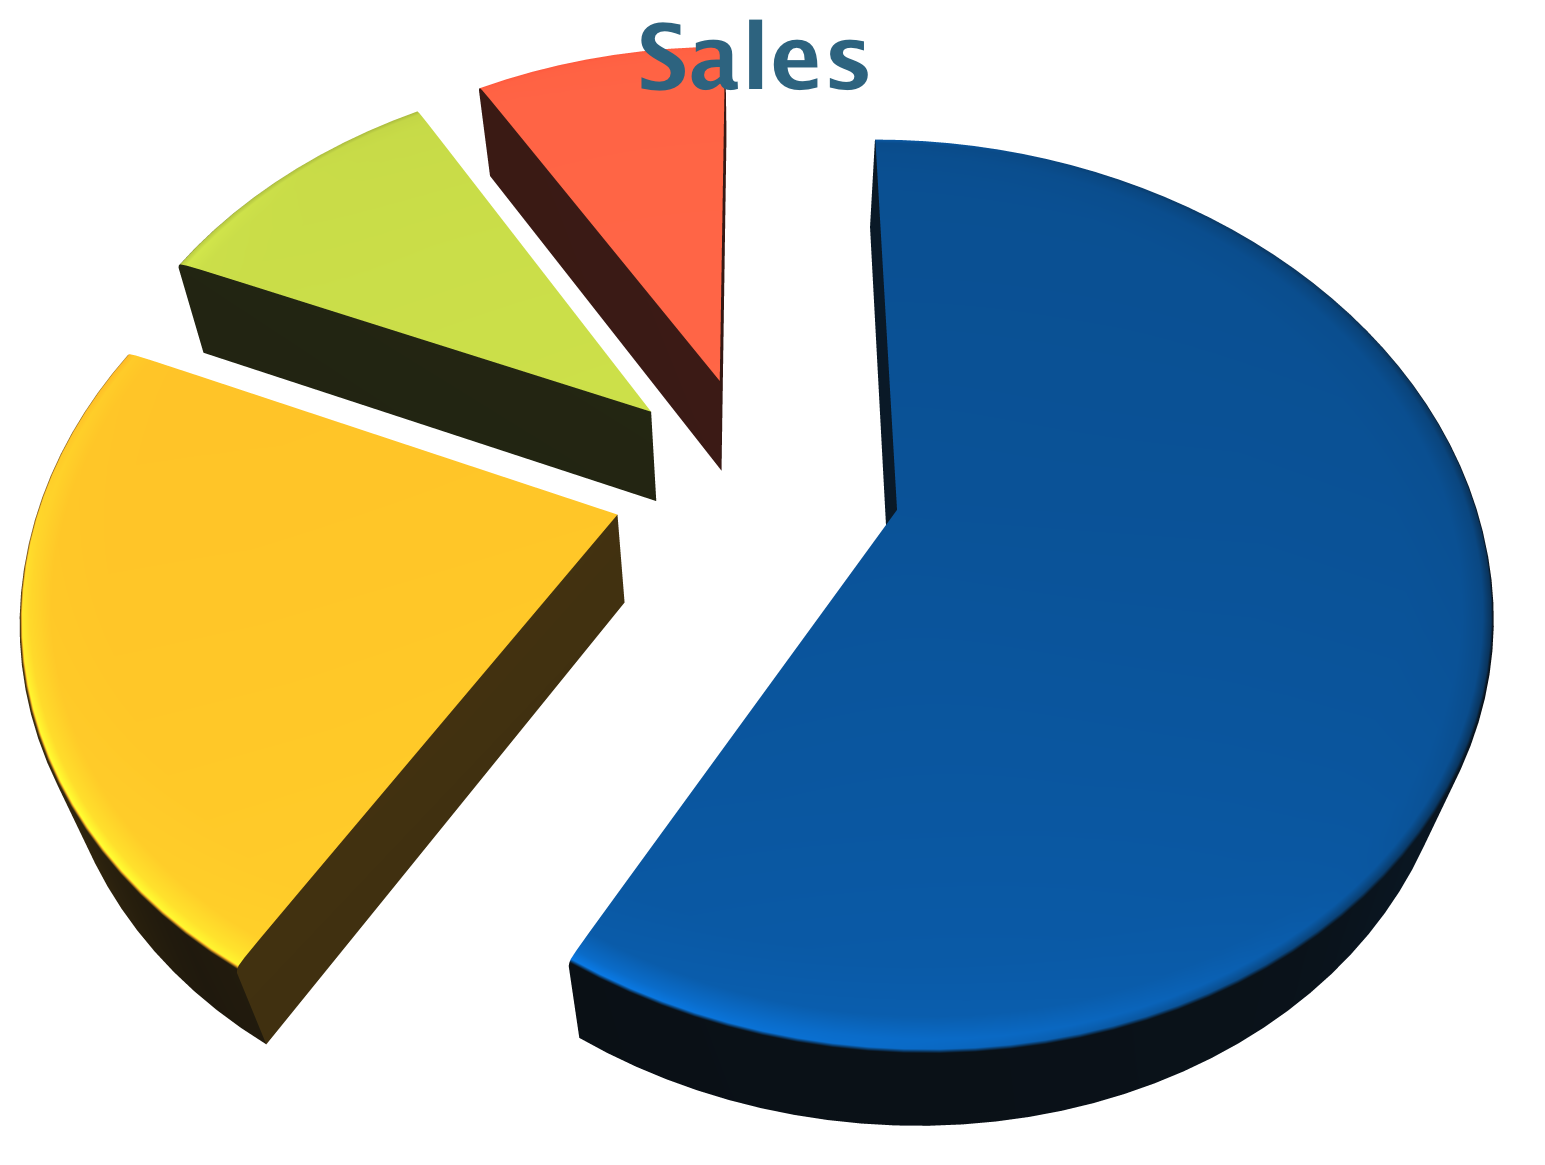
\includegraphics[width=0.4\textwidth]{chart}
\caption{\label{fig:your-figure}ejemplo con una imagen.}
\end{figure}
\end{frame}

\begin{frame}
\frametitle{Text in Two Columns}

\begin{columns}[T]

\begin{column}{0.48\textwidth}
\small
Lorem ipsum dolor sit amet, consectetur adipiscing elit. Fusce sit amet massa in dolor pellentesque tempor. Integer nunc. 
\end{column}

\begin{column}{0.48\textwidth}
\begin{itemize}
\item First bullet goes here
  \begin{itemize}
  \item Secondary bullet goes here
    \begin{itemize}
    \item Tertiary bullet goes here
    \end{itemize}
  \end{itemize}
\end{itemize}
\end{column}

\end{columns}
\end{frame}

\begin{frame}
\begin{figure}[posicion1]
\centering

\includegraphics[width=1.01\textwidth,height=.80\textheight]{gracias}
\end{figure}
\end{frame}
\end{document}